\chapter{Higher Order Applications: Multiple Object Tracking}

As the final aim of my thesis, I am going to inspect the performance of the chosen object detectors on a higher-order problem, namely multiple object tracking. First I am going to review the problem itself, and the common metrics used to measure its performance. 

After this, I will elaborate on the object tracking method I chose as the basis, showing how it incorporates the aforementioned detectors, and the way the performance of the latter is expected to influence tracking performance.

\section{The problem and possible approaches}

Multiple object tracking (MOT) consists of determining the \textit{trajectory} of given kinds of objects in a video stream. In the current context, the trajectory of a single, unique object is a series of bounding boxes with an identifier, one box for every frame in which the object is visible. The rectangular bounding boxes are expected to fit the object shilouette as tightly as possible.

Along the years, several approaches have been developed for the problem, but with the advent of highly accurate object detectors (most notably the breakthrough of convolutional neural networks from the mid-2010s and onward), the detection-based paradigm has become one of the most popular.

The approach consists of detecting objects on each new frame, then assigning them to previously found trajectories, if the object has been seen before, or registering a new trajectory otherwise. This is generally called the \textit{association step}. In some scenarios, when the objects of interest are densely packed, this can pose a considerable difficulty.

Among some popular solutions to this association problem are the \textit{proximity-based} (the Simple Online and Realtime Tracking (SORT) architecture~\cite{Bewley_2016} is one example) and the \textit{feature-based} (the DeepSORT architecture \cite{DeepSORT} incorporates such methods using \textit{deep appearance descriptors}) assignments. The former considers each already existent trajectory, takes their previous location, or the predicted location for this time step, and does the assignment based on some spatial distance between these and current detections. The latter does overarching associations based on visual appearance features, not necessarily restricted to the appearance observed in the last few frames.

The weakness of the proximity-based approach is when the density of objects is high, their movement highly dynamic and their trajectories intertwined. In this case, feature-based methods might excel. The weakness of the feature-based methods might show when they confuse similar, but distinct objects, or when they cannot account for some drastic, fast changes in appearance (like changes in lighting, orientation, deforming, or partial occlusion). In these situations, assignment to last known locations can help. Thus, these two approaches are not, and should not be exclusive.

The introduction above focuses on paradigms and aspects mostly relevant for my thesis, and narrows down the field somewhat. For a comprehensive, recent overview of the problem, see the literature review at~\cite{Luo_2021}. It goes beyond just the detection-based approach, and also formalises the general problem.

Finally, it is worth mentioning that the most common multi-object tracking targets are pedestrians, faces and vehicles, and thus most popular MOT datasets consist of these. In this thesis, I am going to tackle tracking vehicles in road traffic footages.

\section{Metrics [WORK IN PROGRESS]}

When it comes to define metrics to measure a tracking solution's performance, there does not seem to be one trivial, immediately obvious score that can quantify the overall adequacy. When chosing metrics, I had to look for what the most well-known and respected benchmarks measured.

One of, if not the most popular multiple object tracking benchmark is the MOTChallenge\footnote{\url{https://motchallenge.net/}}, introduced in~\cite{MOT15}.

TODO: The MOT15 data format.

\section{SORT, theoretical background [WORK IN PROGRESS]}


\section{Choosing the data}

I will evaluate the model's performance for multi-object tracking on the UA-DETRAC dataset\footnote{\url{https://detrac-db.rit.albany.edu/}}. The dataset contains 100 videos (60 for training, 40 for testing) of road traffic captured at different locations in China. The total length of the video footage is around 10 hours, stored frame by frame (as separate 960 pixel by 540 pixel JPEG images), at the rate of 25 frames per second.

The annotations contain information about vehicle type, illumination, scale (proportional to the square root of the bounding box area), occlusion ratio (the measure by which other objects occlude the vehicle) and truncation ratio (the degree of the bounding box lying outside the frame). Information about weather conditions e.g.~rainy, cloudy, sunny etc.~is also included.


\section{Data Exploration}

At the time of writing this thesis, the test and train images, grouped into sequences that form videos, can be accessed through the Download page of the official site\footnote{\url{https://detrac-db.rit.albany.edu/download}} as \verb|DETRAC-train-data.zip|. However, the tracking annotations for the train and test sets cannot be downloaded, as clicking on the links triggers a popup prompting to log in first. As the login functionality currently does not work, I had to look for alternative ways to access the data.  

Fortunately, after a short search I have found a GitHub repository owned by the Georgia Tech Database Group. Their Exploratory Video Analytics System (EVA) repository contains, among others, a guide on how to download the UA-DETRAC dataset\footnote{\url{https://github.com/georgia-tech-db/eva/tree/master/data/ua_detrac}}, along with a bash script serving the same purpose.

Through those links, I could download the training annotations. Sadly, the test annotations, claimed on the official UA-DETRAC website to be released, were still nowhere to be found, but I figured the 60 sequences (or even a subset of them) should be enough to evaluate tracking performance. The integrity of the measurement wouldn't have been compromised either, as I wasn't planning on doing detector training or hyperparameter tuning on the train set. There were two kinds of training annotation formats provided: XML and MAT.

The XML annotations are meant for detection training, and contain additional information like vehicle category, weather conditions during filming and bounding box scale. I did not use this data directly, as I used the models pre-trained on the COCO dataset, but inspecting this data confirms the vehicle categories supported by the DETRAC dataset: \textit{car}, \textit{van}, \textit{bus}, \textit{other}. The corresponding COCO object categories are \textit{car}, \textit{truck}, \textit{bus}, so that is what I will be looking for when runnning detection on the images, and ignoring all other classes.

The MAT annotations are files in MATLAB serialization format, containing trajectory and position information for all tracked entities. For every image sequence, there is a \verb|MVI_NNNNN.MAT| file.
The image sequences themselves are consecutive frames under \verb|Insight-MVT_Annotation_Train/MVI_NNNNN|, after unzipping \verb|DETRAC-train-data.zip|.

Initially I inspected the MAT files' inner structure (see figure~\ref{fig:octave-exploration}) in GNU Octave, MATLAB's open-source and somewhat compatible counterpart. I found that each file contained 5 matrices:
\begin{enumerate}
    \item{$X$: An $N \times T$ matrix, where $T$ is the number of trajectories, and $N$ is the number of frames. Given the frame $i$ and trajectory $j$, $x_{i,j}$ denotes the $x$ coordinate of the bottom center of the bounding box\footnote{I found this out initially through trial and error, when trying to visualize bounding boxes in Python, because I did not know this to be a common format for specifying bounding boxes. Later, I found it mentioned in \url{https://detrac-db.rit.albany.edu/FAQ} as \textit{foot position}.}, or $0$ if trajectory $j$ is not present in that frame.}
    \item{$Y$: An $N \times T$ matrix, similar to $X$, but it contains the $y$ coordinates of the bounding boxes' foot position.}
    \item{$W$: contains the width of the boxes.}
    \item{$H$: contains the height of the boxes.}
    \item{$frameNums$: A row vector of length $N$, containing the 1-based indices of the frames.}
\end{enumerate}

\begin{figure}[h]
    \begin{center}
        \captionsetup{width=0.8\textwidth}
        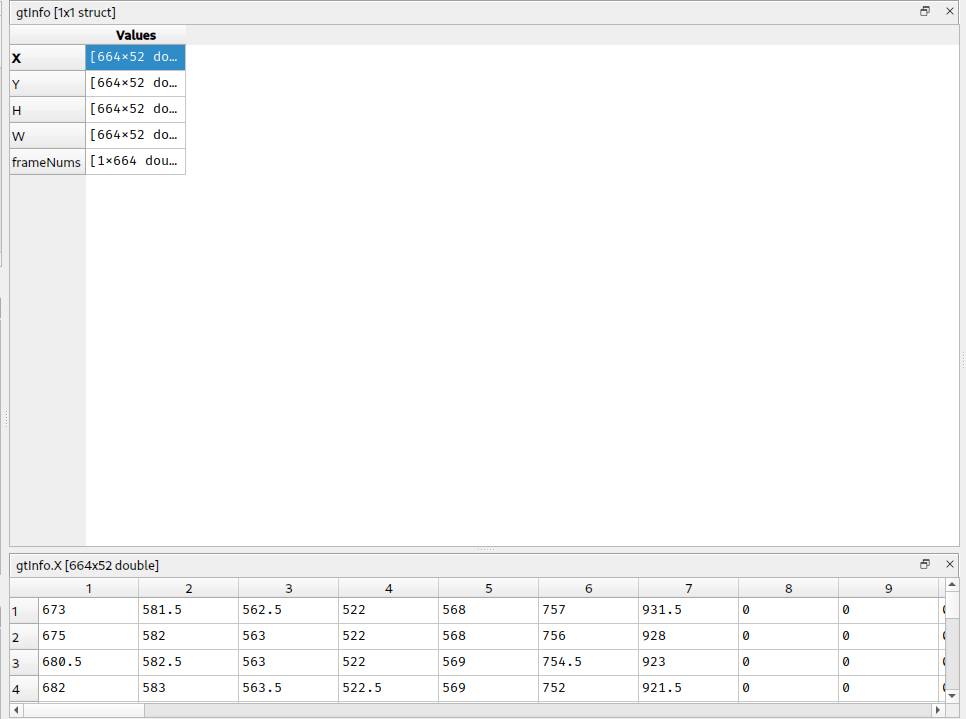
\includegraphics[width=0.8\textwidth]{figures/octave.png}
        \caption{Label data exploration in octave}
        \label{fig:octave-exploration}
    \end{center}
\end{figure}


\section{Benchmark}

The dataset and the benchmark is described in~\cite{CVIU_UA-DETRAC}. The article also proposes an evaluation protocol for multi-object tracking. A key point is the joint analysis of detection and tracking performance, analysing the effects of the chosen model's precision/recall values (and the underlying confidence threshold setting that influences both) in relation with the tracking performance, as reflected by the MOTA and MOTP score. These relationships are visualized on the PR-MOTA and PR-MOTP curves (See figure~\ref{fig:pr-mota}).

\begin{figure}[h]
    \captionsetup{width=\textwidth}
    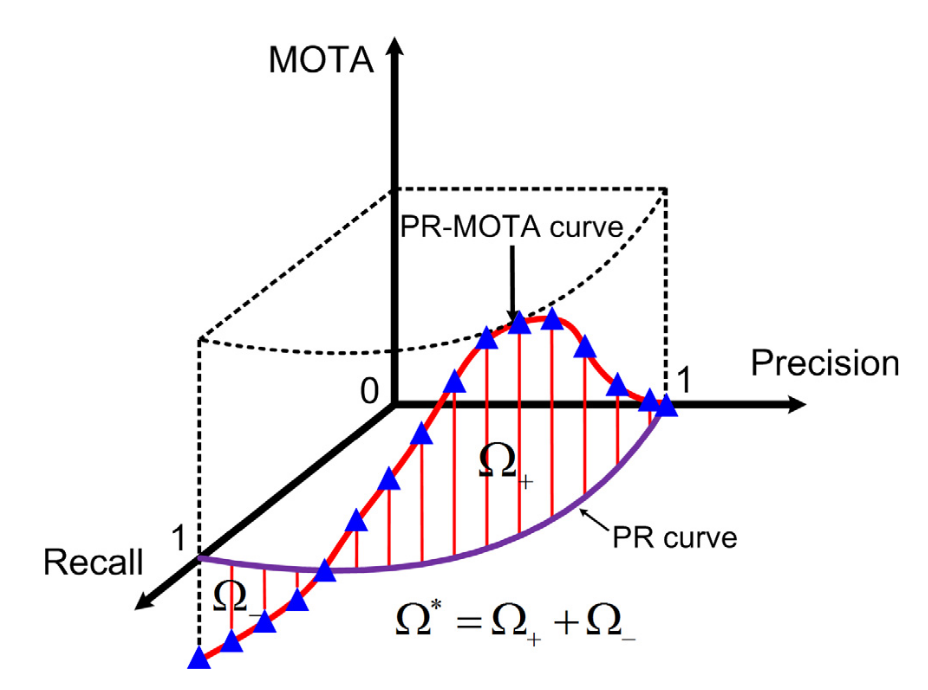
\includegraphics[width=\textwidth]{figures/pr-mota-curve.png}
    \caption{Visualization of the PR-MOTA curve. Image taken from \cite{CVIU_UA-DETRAC}}
    \label{fig:pr-mota}
\end{figure}

The authors argue that, as it is not fair, nor enough to compare the performance of two object detectors based on different points on the PR curve, it is also not enough to determine the maximum point on the PR-MOTA curve, as a good tracker must produce good scores in a wider range of settings. The whole range of the curve must be taken into account in some form, thus the need for a new metric, $\Omega^{*}$, or the \textit{PR-MOTA score}:

\[ \Omega^{*} = \frac{1}{2}\int_{\mathcal{C}} \Psi(p, r) \,d\textbf{s} \]

where $\Psi$ is the MOTA score across the whole dataset at precision $p$ and recall $r$, and we calculate the (approximate value of the) signed area under the PR-MOTA curve as an integral along the PR curve $\mathcal{C}$ (for every $(p, r) \in \mathcal{C}$). Dividing by 2 ensures that the score stays in the interval $(-\infty, 100\%]$. Similar metrics can be defined for the MOTP, FP, FN, IDS, MT and ML scores.

\section{Designing the measurement}

For the measurment, I chose 7 detectors in total: two DETR variants, one with the ResNet50 and one with the ResNet101 backbone, pre-trained on the COCO 2017 dataset. The other 5 were the YOLOv5n (nano), YOLOv5s (small), YOLOv5m (medium), YOLOv5l (large), YOLOv5x (extra large). These differ in the size, as in number of parameters, and this influences the inference times as well.

Each detector was evaluated at 10 confidence thresholds: from 0.0 to 0.9, incremented by 0.1.

To calculate the value defined by the UA-DETRAC benchmark, I had to break the process into multiple steps and assess the best tool for each subtask.

As input data, I had the UA-DETRAC training videos, as frame sequences, and the annotations in MATLAB format.

For my tracker of choice, I could clone the public GitHub repository\footnote{\url{https://github.com/abewley/sort}}, and run the tracker, provided I put the detections in MOT2015 format for each sequence under the \verb|data| folder.

The rest of the steps had to be implemented by me. First, I had to create a model executor that returned the detections from each frame of the video sequences, and served as a adapter-wrapper around both the DETR and the YOLOv5 models, to hide the differences in preprocessing. I invoked this this on all combinations of models, confidence thresholds and sequences. For each unique trio of these, one file has been saved in the MOT15 detection format.

The detections themselves, along with the annotations were enough to calculate the precision-recall curve for each model, aggregating the values for all sequences. For evaluation I used the standard IoU metric for ground truth-prediction distance, with IoU threshold 0.7 (In the code, \verb|max_iou| is set to 0.3, because the library I used considers $1-IoU$ when matching ground truth with prediction. More on that in the relevant subsection). This is not to be confused with the confidence threshold, which is a property of the detector that can be set, and varies. This is a global setting which means that a good prediction can be considered a match to the ground truth box only if their IoU distance is at least 0.7, a reasonable expectation according to my visual intuition.

Next, I ran the SORT script provided in the official repository for each model separately, on every sequence and confidence threshold combination. These were automatically saved in the MOT15 tracking annotation format.

Having the tracking output and the ground truth annotations, I ran the tracking evaluation on every model and confidence threshold combination, aggregating MOTA values for all sequences. The evaluation IoU threshold was set to 0.7, like at the detection evaluation.

Given both the precision-recall curves for every model (where both precision and recall are a function of the confidence threshold), and the MOTA values for every model and confidence threshold combination, I could finally calculate the PR-MOTA scores for each model.

A visual overview of the process above can be seen in figure~\ref{fig:workflow}. Detailing of the individual design choices made at each step can be found in the following subsections. At some of the steps, I implemented visualizations as a way to spot possible errors in implementation that could compromise the whole measurement. 

The language I used was Python 3.10, the inference times were recorded under Linux, on a desktop PC with an AMD Ryzen 3800X processor, 32 Gigabytes of RAM and an RTX3060Ti graphics card with 8 Gigabytes of VRAM. 

\begin{figure}[h]
    \captionsetup{width=\textwidth}
    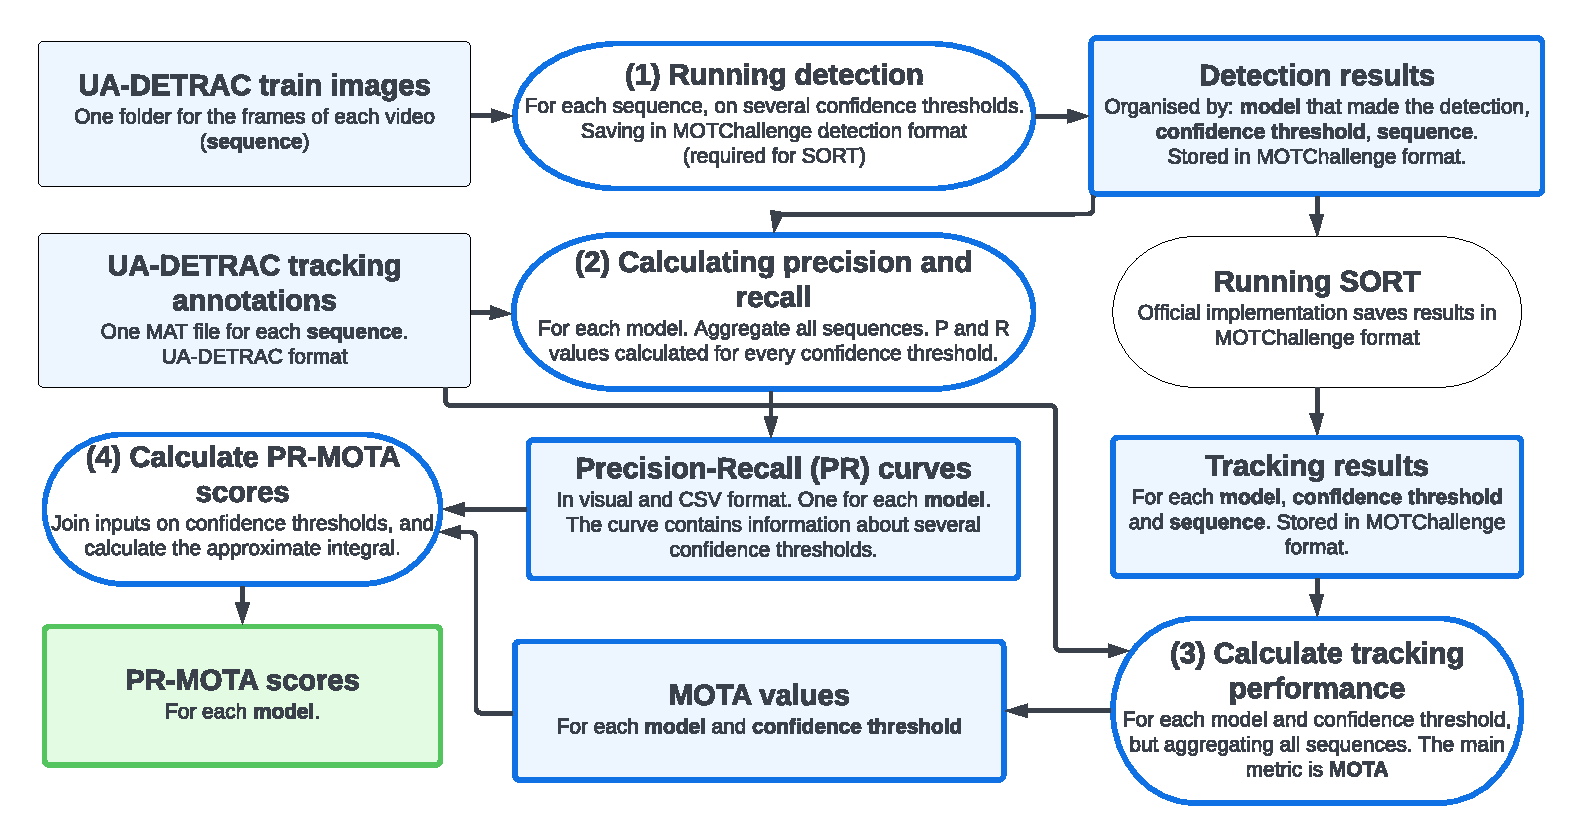
\includegraphics[width=\textwidth]{figures/workflow.pdf}
    \caption{Flowchart visualization of my workflow. The blue rectangles denote data, rounded rectangles denote processing steps. Blue outline means that part of the workflow was implemented by me, or the data was generated in the process. No blue outline means either the data is from an external source, or the processing step involved using entirely external code.}
    \label{fig:workflow}
\end{figure}

\subsection{Running the detections}

In order to evaluate the aforementioned models on images, I had to find the easiest way to load the pretrained weights for each model.

For the DETR, the \verb|transformers| Python package by Huggingface\footnote{\url{https://huggingface.co/docs/transformers/index}} provides the easiest API, with simple pre- and postprocessing (including confidence thresholding and converting from logits to probability distributions), and also provides a way to download pretrained weights. Under the hood, \verb|transformers| uses a PyTorch \verb|torch.nn.Module|, so sending it to the GPU is similar to all Torch modules. Also theoretically loading from Torch Hub was also a possibility, but the pre- and postprocessing tasks would have been messier.

As for the YOLOv5 model, it can be loaded directly from Torch Hub, and its input format is way more flexible, so lists of images (for the inference, I used batches of size 1), but even image links can  be fed to it directly.

To hide the differences between these two approaches, I implemented an adapter class for them, and also added visualization capabilities to spot possible errors in the interpretation of data (for example, assuming wrong bounding box format).

I also wanted to meausre average inference times to show a picture about the real time capabilities of each detector. All inference happened on the GPU, so due to the asynchronous nature of the Torch CUDA operations, measuring elapsed time on CPU was out of the question. The appropriate time measuring method, as suggested on the official Torch forums\footnote{\url{https://discuss.pytorch.org/t/how-to-measure-time-in-pytorch/26964}} was through the \verb|torch.cuda.Event| object. I took the elapsed GPU time between the moment of feeding the inputs until recieving the logits, but this didn't include copy times between the RAM and VRAM, neither the postprocessing steps (calculating probability distributions with softmax, confidence thresholding).

Timing results can be seen in table~\ref{tab:inference-times}. All code to reproduce the results can be found on the GitHub repository of my thesis\footnote{
    See \url{https://github.com/peter-i-istvan/bsc-thesis}, under \texttt{tracking/run\_detection.py}.
}.

\begin{table}[h]
    \begin{tabular}{|c|c|c|c|c|c|c|c|}
        \hline
         & yolov5n & yolov5s & yolov5m & yolov5l & yolov5x & detr-resnet-50 & detr-resnet-101 \\
        \hline
        \hline
        avg (ms) & 7.38 & 7.38 & 8.99 & 12.00 & 20.88 & 43.98 & 64.53 \\
        \hline
        std (ms) & 1.16 & 0.24 & 0.24 & 0.18 & 0.27 & 0.80 & 0.66 \\
        \hline
        \hline
            FPS & 135.5 & 135.5 & 111.2 & 83.3 & 47.89 & 22.73 & 15.49 \\
        \hline
    \end{tabular}
    \caption{Average inference times on GPU and their standard deviation (expressed in miliseconds) for each model, after running on every sequence.}
    \label{tab:inference-times}
\end{table}

\begin{figure}[h]
    
\end{figure}

\subsection{Calculating precision and recall}

Next, I had to calculate precision and recall curves for the detections. To do this, for every model and confidence threshold pair, I had to sum all true positives, false positives and false negatives in every sequence. For the theoretical definition of these, not only in the general meaning, but in the case of object detection, where assignment between ground truth and predicted boxes is not always trivial (the Hungarian bipartite graph matching algorithm solves this ambiguity), see chapter one.

For the concrete implementation, I took a `sideways' approach, but one that could be mostly reused later in calculating the MOTA score as well. The \verb|motmetrics| Python package\footnote{\url{https://pypi.org/project/motmetrics/}} provides handy tools for calculating MOT metrics, like those in CLEAR MOT. Specificaly, it gives us an \textit{accumulator} object that must be initialized before evaluating on a seqence, then for each frame, its \verb|update()| function must be called to update its state. In the arguments, one must provide ground truth IDs and predicted IDs, as well as a distance matrix that expresses the distance between ground truth box \textit{i} and prediction box \textit{j}. In theory, \verb|motmetrics| is distance-agnostic, which means that any kind of distance can be supplied, but I used the IoU box distance metric, which is one of the most popular evaluation metrics both for object detection and multiple object tracking. \verb|motmetrics| provides functions for calculating all popular metrics, so incorporating IoU calculation into my code was easy.

In its update step, the accumulator takes the input arguments, and in the first parts, it is not at all concerned with the IDs provided, but calculates the best ground truth box-to-prediction assignment with the Hungarian algorithm. This is the very exact action that is needed at detection evaluation as well, this is why we `piggy-backed' tracking evaluation. Based on this assignment, it generates \verb|MATCH|, \verb|MISS| and \verb|FP| events, which correspond to true positives, false negatives and false positives respectively.

In the next steps, if we provided valid prediction IDs (a.k.a our hypotheses for the identities of the tracked objects), the accumulator would also record possible mistakes with regard to identity confusion, like identity swaps. However, considering that the MOTChallenge format defines -1 as the ID field when saving only detections, not tracking results, technically we tell the accumulator that all found boxes correspond to our object -1, which makes the rest of this step absolute rubbish, but it does not influence the events already recorded in the first step, and in the first steps of all future update calls.

After finishing a sequence, the script extracts the number of relevant events, and adds them to all the previously calculated occurrences of true positives, false negatives and false positives for that model-confidence threshold pair. At the end of this, we will have a mapping counting all of these for every sequence. Then I iterate through all model-confidence threshold pairs, calculate the precision and recall values given by the formulas:
\[P = \frac{TP}{TP + FP}\]
\[R = \frac{TP}{TP + FN}\]

Finally, I save them as CSV files. The result can be seen in tables~\ref{tab:p_curve} and~\ref{tab:r_curve}.

\begin{table}
    \begin{centering}
    \begin{tabular}{|c||c|c|c|c|c|c|c|}
        \hline
        CT & D101 & D50 & YL & YM & YN & YS & YX \\
        \hline
        \hline
        0.9 & 0.52 & 0.47 & 0.93 & 1.0 & 1.0 & 0.90 & 0.64 \\
        \hline
        0.8 & 0.45 & 0.41 & 0.54 & 0.61 & 0.83 & 0.61 & 0.49 \\
        \hline
        0.7 & 0.40 & 0.37 & 0.54 & 0.51 & 0.68 & 0.52 & 0.46 \\
        \hline
        0.6 & 0.36 & 0.33 & 0.51 & 0.46 & 0.53 & 0.45 & 0.44 \\
        \hline
        0.5 & 0.33 & 0.30 & 0.46 & 0.42 & 0.42 & 0.39 & 0.41 \\
        \hline
        0.4 & 0.30 & 0.28 & 0.40 & 0.37 & 0.34 & 0.32 & 0.36 \\
        \hline
        0.3 & 0.28 & 0.26 & 0.33 & 0.31 & 0.28 & 0.27 & 0.30 \\
        \hline
        0.2 & 0.25 & 0.23 & 0.30 & 0.28 & 0.25 & 0.24 & 0.27 \\
        \hline
        0.1 & 0.21 & 0.21 & 0.30 & 0.28 & 0.25 & 0.24 & 0.27 \\
        \hline
        0.0 & 0.19 & 0.18 & 0.30 & 0.28 & 0.25 & 0.24 & 0.27 \\
        \hline
    \end{tabular}
    \caption{The precision curve of the models. CT is confidence threshold, D101 and D50 is DETR-Resnet 101 and 50, while YL, YM, YN etc. are the yolo versions.}
    \label{tab:p_curve}
    \end{centering}
\end{table}

\begin{table}
    \begin{centering}
    \begin{tabular}{|c||c|c|c|c|c|c|c|}
        \hline
        CT & D101 & D50 & YL & YM & YN & YS & YX \\
        \hline
        \hline
        0.9 & 0.63 & 0.57 & 0.03 & 0.01 & 0.00 & 0.02 & 0.12 \\
        \hline 
        0.8 & 0.69 & 0.65 & 0.41 & 0.34 & 0.13 & 0.36 & 0.46 \\
        \hline 
        0.7 & 0.71 & 0.68 & 0.59 & 0.52 & 0.41 & 0.56 & 0.60 \\
        \hline 
        0.6 & 0.73 & 0.69 & 0.69 & 0.63 & 0.52 & 0.66 & 0.69 \\
        \hline 
        0.5 & 0.73 & 0.71 & 0.76 & 0.72 & 0.60 & 0.72 & 0.76 \\
        \hline 
        0.4 & 0.74 & 0.71 & 0.81 & 0.79 & 0.66 & 0.77 & 0.81 \\
        \hline 
        0.3 & 0.75 & 0.72 & 0.84 & 0.84 & 0.70 & 0.80 & 0.84 \\
        \hline 
        0.2 & 0.75 & 0.72 & 0.86 & 0.86 & 0.72 & 0.81 & 0.86 \\
        \hline 
        0.1 & 0.76 & 0.73 & 0.86 & 0.86 & 0.72 & 0.81 & 0.86 \\
        \hline 
        0.0 & 0.76 & 0.73 & 0.86 & 0.86 & 0.72 & 0.81 & 0.86 \\
        \hline
    \end{tabular}
    \caption{The recall curve of the models. CT is confidence threshold, D101 and D50 is DETR-Resnet 101 and 50, while YL, YM, YN etc. are the yolo versions.}
    \label{tab:r_curve}
    \end{centering}
\end{table}

Running this took 1 hour and 8 minutes on my machine. For implementation, see my GitHub repository\footnote{See \url{https://github.com/peter-i-istvan/bsc-thesis}, under \texttt{tracking/detection\_evaluation.py} for the code, \texttt{p\_curve.csv}, and \texttt{r\_curve.csv} for the curves in }, where the curves are also available, saved in CSV format. 

\textbf{insert plots when ready}

\subsection{Running SORT}

I ran SORT by cloning its repository, applying a small patch to account for divison by 0 at empty detection files (happened with YOLOv5n models for some sequences, at high confidence thresholds), installing the dependencies and issuing the following command:
\begin{verbatim}
    python sort.py --seq_path DETECTIONS_ROOT --phase MODEL --max_age 3
\end{verbatim}

The main hyperparameters of SORT are \verb|min_hits|, \verb|max_age| and \verb|iou_threshold|, all of them can be supplied to the script by command line parameters.

Minimum hits means the minimum number of consecutive times a new trajectory must be confirmed (by detection `hits' that get assigned to it) to consider it a real one. Its default value is 3, and I left it at that.

Maximum age is the longest consecutive time that a trajectory without detection (if the detector somehow lost the object) can be kept alive. The position predictions are still updated, so the tracker looks for the object a little bit further apart at each frame, in the direction and considering the magnitude of the last known velocity. The default value is 1, but I set it to 3 because it seemed reasonable (based on my experiences in the Project Laboratory course, where similar maximum ages lead to better results).

IoU threshold is the minimum IoU value between the hypothesized current bounding box location of the object (predicted by the Kalman filter) and any detection bounding box that can be matched with it. The default value is 0.3, and I left it at that.

During the consecutive runnings of the script, I recorded the elapsed time and FPS reported by the script for each model. The results are confirming the belief that SORT is a very fast tracker, with the main factor for the tracking framerate in a real time scenario (where detections are not precomputed) being the detection time (almost two orders of magnitude higher than the tracking time at each frame). For the results, see table~\ref{tab:sort-times}.

\begin{table}[h]
    \begin{tabular}{|c|c|c|c|c|c|c|c|}
        \hline
         & yolov5n & yolov5s & yolov5m & yolov5l & yolov5x & detr-resnet-50 & detr-resnet-101 \\
        \hline
        \hline
        Time (s) & 1313.99 & 1155.18 & 482.8 & 599.88 & 611.18 & 654.18 & 668.11\\
        \hline
        \hline
        FPS  & 637 & 725 & 1710.2 & 1391.7 & 1369.1 & 1279.1 & 1253.5 \\
        \hline
    \end{tabular}
    \caption{Statistics reported by the SORT script. The evaluation was done on 60 videos and on 10 confidence thresholds, making a total of 600 detection inputs. The time is the total evaluation time for all 600 inputs. The numbers are aggregated over confidence thresholds, but on lower values, tracking tends to take more time, as the consistent erroneus detections form a high number of false tracks.}
    \label{tab:sort-times}
\end{table}

\subsection{Calculating tracking performance}

\subsection{Calculting benchmark scores}

\section{Conclusion}

% \subsection{Evaluation}

% The tracking evaluation toolkit on the official DETRAC website is not available\footnote{\url{https://detrac-db.rit.albany.edu/Tracking}, under DETRAC-toolkit (Windows beta)}, because the login feature does not work. Thus, I had to write my own implementation for the evaluation based on the CLEAR MOT metrics~\cite{Bernardin2008}.



% \subsection{Running the detections}

% For the detectors, I have chosen the Detection Transformer (DETR) model as a representative Transformer-based architecture, with two variants, containing the ResNet50 and the ResNet101 backbones, pre-trained on the COCO 2017 dataset.

% On the Fully Convolutional Network (FCN) side, I have chosen a rendition of the You Only Look Once (YOLO) architecture that came out at roughly the same time as the DETR: the YOLOv5. The official repository of the YOLOv5 project\footnote{\url{https://github.com/ultralytics/yolov5}} contains five pre-trained variants: the YOLOv5n (nano), YOLOv5s (small), YOLOv5m (medium), YOLOv5l (large) and YOLOv5x (extra large), all being trained on the COCO 2017 dataset.

% Before running the SORT tracker, I had to prepare the detection results for all sequences in a specific format.



% \subsection{Running the tracker}

% \begin{figure}[h]
    % \captionsetup{width=\textwidth}
    % \includegraphics[width=\textwidth]{}
    % \caption{...}
    % \label{fig:dunno}
% \end{figure}

% \subsection{Tracking visualisation}


% \subsection{Rest}

% Usually, a baseline for detection performance in MOT is the R-CNN architecture and its variants.

% For the MOT task, I have chosen the SORT architecture, introduced in~\cite{Bewley_2016}. Altough not the most recent, it is the architecture I have examined in my project laboratory, and has the analytical advantage of solely relying on detection performance, as opposed to method like DeepSORT that are influenced by the association method as well. It can be considered a reasonable baseline methood, relying on first-order velocity estimation and smoothing measurement errors based on the Kalman Filter.  